%!TEX root=./pfc.tex
\chapter[Pruebas del sistema]{Pruebas del sistema}

La fase de pruebas es una fase primordial para garantizar la fiabilidad de un sistema, debido a que representa un último repaso a las especificaciones, al diseño y a la implementación del mismo.
Esta parte de la documentación pretende realizar una descripción de las pruebas realizadas al software desarrollado y cuyos correctos resultados permitirán asegurar que el sistema satisface los requisitos impuestos y cumple con los objetivos deseados de manera robusta y eficiente.

\section{Objetivos de las pruebas}

Las pruebas son una actividad en el desarrollo del software en la cual el sistema o alguno de sus componentes se ejecutarán en circunstancias previamente especificadas, observando y registrando los resultados para realizar una evaluación de algún aspecto. Probar es el proceso de ejecutar un programa con el fin de encontrar errores.

En este caso, la prueba exhaustiva del sistema software con el que se trata resulta perfectamente viable debido a que se pueden probar con facilidad todas las posibilidades de su funcionamiento sin incurrir en ningún error. Por ello se plantean una serie de puntos generales para este proceso:

\begin{itemize}
	\item El objetivo es realizar pruebas que delaten distintos errores con poco tiempo y esfuerzo.
	\item Secundariamente demostraremos con las pruebas qué módulos del software funcionan de acuerdo a las especificaciones y requisitos dados. El comportamiento de la aplicación nos indicará qué grado de fiabilidad tiene el programa y su calidad.
	\item Por último, hay que tener en cuenta que las pruebas no aseguran la falta de defectos. Sin embargo, si todo esto resultara ineficiente, se ha de recordar que tras esta fase de pruebas se lleva a cabo una etapa de explotación del sistema, con la peculiaridad de que éste se dispondrá a funcionar en el entorno propio y real de la aplicación pero bajo la supervisión y controlado por los encargados directos del mismo, pudiendo observar si verdaderamente el programa esta listo para su definitiva aceptación.
\end{itemize}

\section{Diseño de los casos de pruebas}

Analizando las especiales características del software, se llega a la conclusión de que es necesario prestar especial atención a:

\begin{itemize}
	\item Asegurar la comunicación entre el módulo de Moodle y el sistema encargado de sincronizar el código y programar los bloqueos. Esta comunicación es la base del sistema por lo que deben estar completamente sincronizados de manera que cada petición sea servida convenientemente. Además, cada cambio en el editor introducida en el cliente debe ser indicada al servidor para que este se encargue de sincronizarlo con el resto de usuarios.
	\item Garantizar la correcta visualización de las pantallas, fundamentalmente la de edición.
	\item Garantizar el correcto acceso a la base de datos, ya sea para obtener cualquier dato de la comunidad como para almacenar y recuperar los datos referentes a la sincronización del código.
	\item Asegurar que un usuario no puede modificar una parte bloqueada por otro usuario, ya sea por error suyo o problemas en el sistema.
	\item Asegurar el correcto funcionamiento de todas las demás opciones posibles.
\end{itemize}

\section{Pruebas estructurales de la caja blanca}

Aprovechando que tanto Java como PHP permiten una sencilla y cómoda interpretación de código, gracias sobre todo a las potentes herramientas que existen para cada una de ellas y que se comentaron en el apartado de recursos software, se ha ejecutado el código al completo haciendo énfasis en bucles y condiciones forzando dicha ejecución en todas aquellas partes de código que por un motivo u otro no suelen ser accedidas. Gracias a este proceso, se han descubierto algunos fallos en dichas zonas que han sido resueltos convenientemente.

Debido a las características del software que se ha desarrollado, el enfoque de las pruebas que, teóricamente, más errores podrá detectar es el funcional o de la caja negra.

\section{Pruebas funcionales o de la caja negra}

\subsection{Análisis de los valores límites}

Al tratarse de un sistema donde la intercomunicación entre el usuario y este es constante, en este apartado es donde radica el mayor número de pruebas. Como la parte fundamental de este proyecto se trata de un editor, el usuario tiene permitido hacer en él todo lo que desee y prácticamente sin limitación alguna. Sin embargo, para evitar errores se ha impedido al usuario realizar una serie de acciones que podrían poner en peligro la estabilidad del sistema. 

Muchas de estas acciones han sido camufladas como ayuda al usuario, como puede ser por ejemplo que la apertura y cerrado de funciones se hace de modo automático. De este modo, y al ser los bloqueos por funciones, es el sistema el que lo delimita automáticamente y no así el usuario.

Una vez puntualizados estos datos, se van a enumerar una serie de hechos que son candidatos a la realización de pruebas:

\begin{itemize}
	\item Un punto en el que se han hecho pruebas exhaustivas es en el acceso a las partes bloqueadas por otro usuario del código fuente. Asimismo también se ha hecho énfasis en los puntos de sección crítica que puedan concurrir.
	\item Otro punto importante es la llamada al compilador, que al tratarse de una aplicación externa lo hace necesario del uso de ficheros, por lo que se ha evaluado el acceso a estos.
	\item Del mismo modo que el punto anterior también se presta atención al chat, que también trabaja con ficheros, por lo que hay que hacer pruebas exhaustivas para su acceso a estos.
	\item Otras pruebas que se han realizado han sido pruebas a la interfaz del software, es decir, se ha probado que todas las pantallas sean accesibles y que la comunicación entre ellas es eficiente.
\end{itemize}

\section{Pruebas del desarrollador}	
	
Realmente son las pruebas más importantes que se han realizado. Básicamente estas pruebas se han centrado fundamentalmente en tres puntos comentados a continuación.

\subsection{Pruebas con un curso real}	
	
Antes de nada comentar que la utilidad de este software se centra en las comunidades virtuales de aprendizaje en las que la colaboración es su principal objetivo. Si esto no es así, gran parte de la utilidad de esta herramienta se perdería, pues la mayor funcionalidad que expresa es su capacidad de hacer el editor colaborativo en tiempo real. 

Para ello en primer lugar se ha creado un curso en Moodle, dentro del cual un profesor simulado ha ido creado una serie anotaciones y matriculando una serie de alumnos virtuales.

\begin{figure}[h]
	\includegraphics[width=\textwidth]{./img/ej1main.eps}
	\caption{Pantalla principal de un curso Moodle}
\end{figure}
	
Una vez dentro del curso se han creado una serie de Wikicodes diferentes para probar las distintas opciones de configuración. Estas pruebas tienen como principales objetivos:

\begin{itemize}
	\item Realizar una serie de códigos fuentes, tanto individualmente como de modo colaborativo, y luego comprobar si la compilación es correcta.
	\item Si la compilación es errónea, comprobar que las líneas referenciadas son claramente identificadas en el editor dentro de la Wikicode.
	\item Comprobar que todas las acciones que puedan realizarse dentro de un entorno de desarrollo pueden hacerse libremente dentro de una Wikicode, desde la restauración de una versión antigua a desbloquear partes de tu código.
\end{itemize}

Por tanto, dicho curso se ha desarrollado de manera completa y se han creado varios alumnos ficticios los cuales realizaron numerosas aportaciones y colaboraciones en la comunidad. Además, se ha utilizado para probar todas las opciones disponibles intentando barajar todas posibilidades que el usuario podría realizar en el entorno del curso.

\begin{figure}[h]
	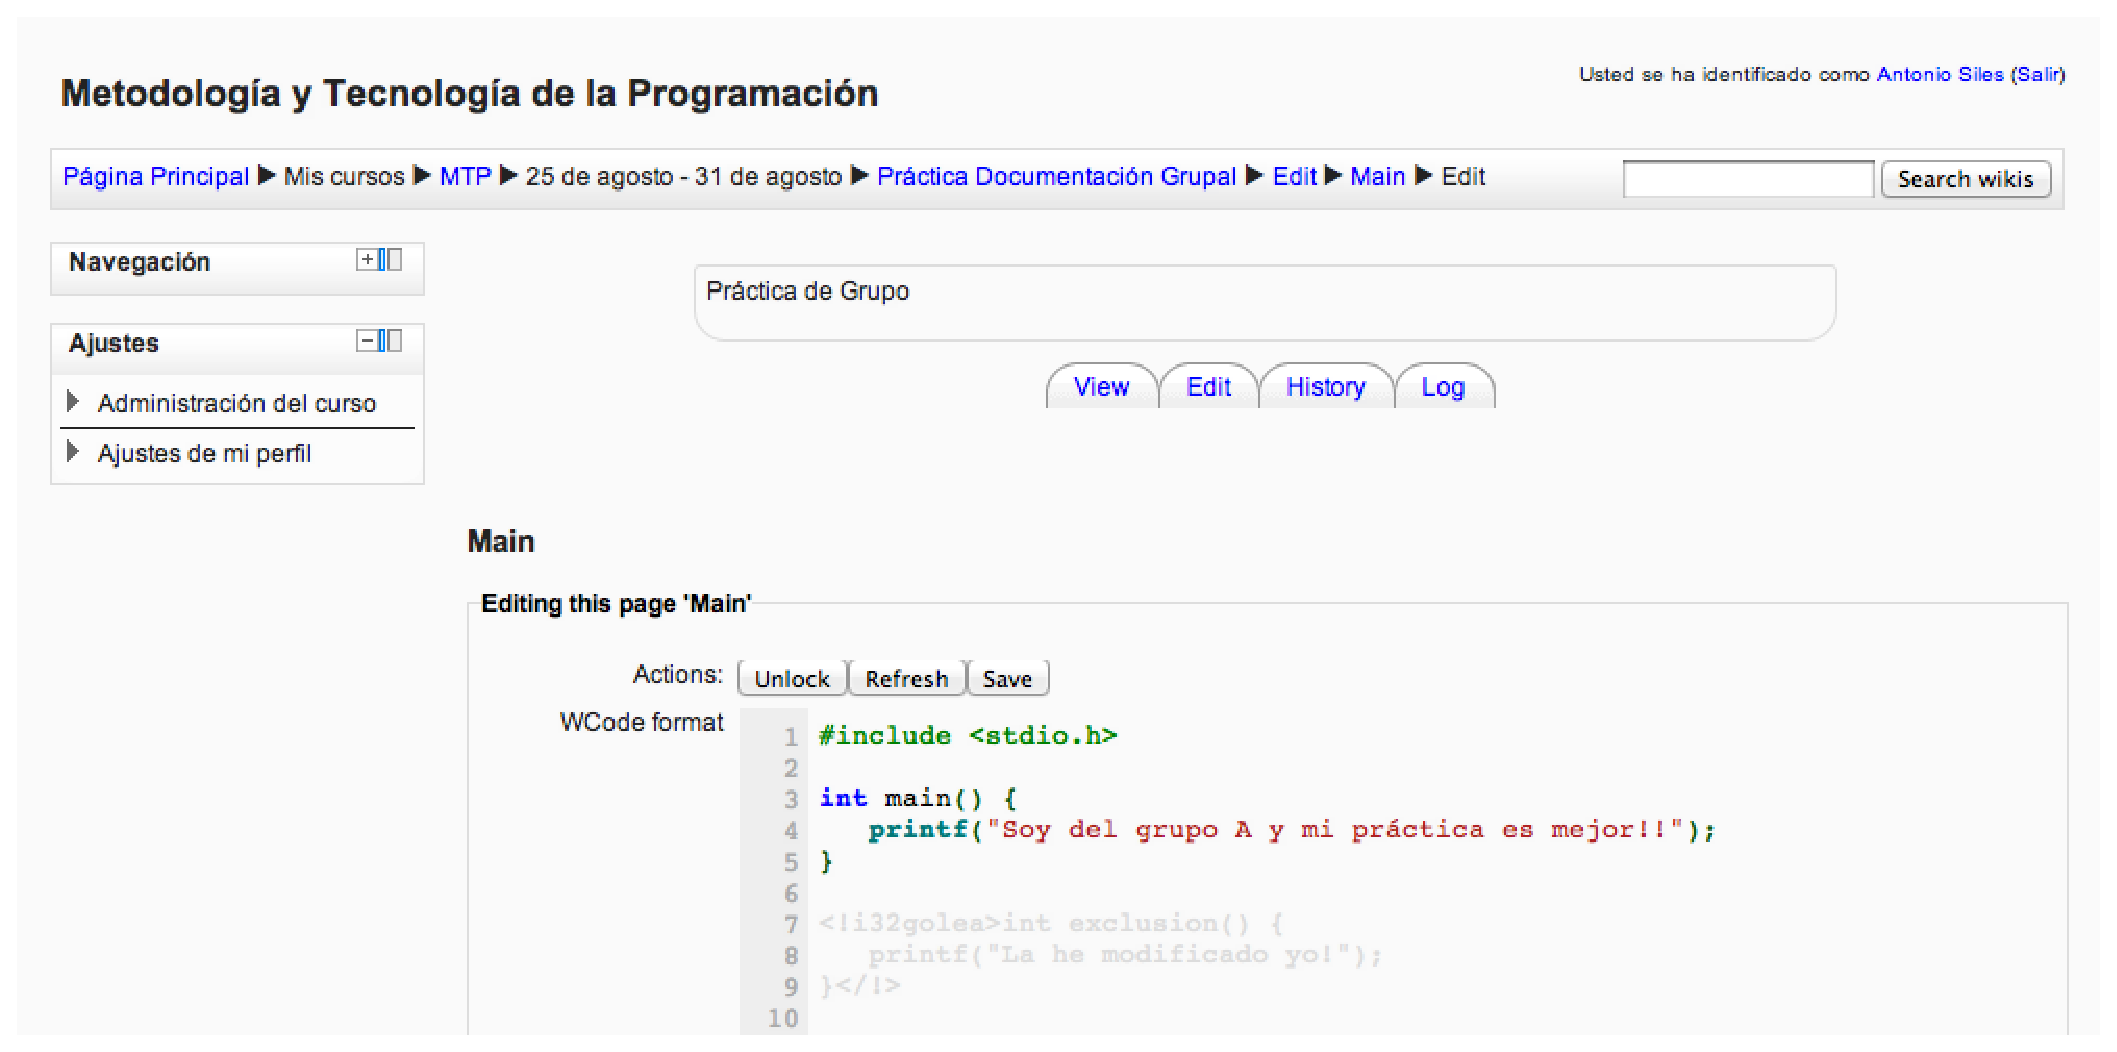
\includegraphics[width=\textwidth]{./img/ej2edit4.eps}
	\caption{Edición de código con una función bloqueada}
\end{figure}

\newpage	
También se ha probado la opción de Descarga del ejecutable una vez compilado y se ha comprobado que se ejecuta correctamente.	
	
\begin{figure}[h]
	\centering
	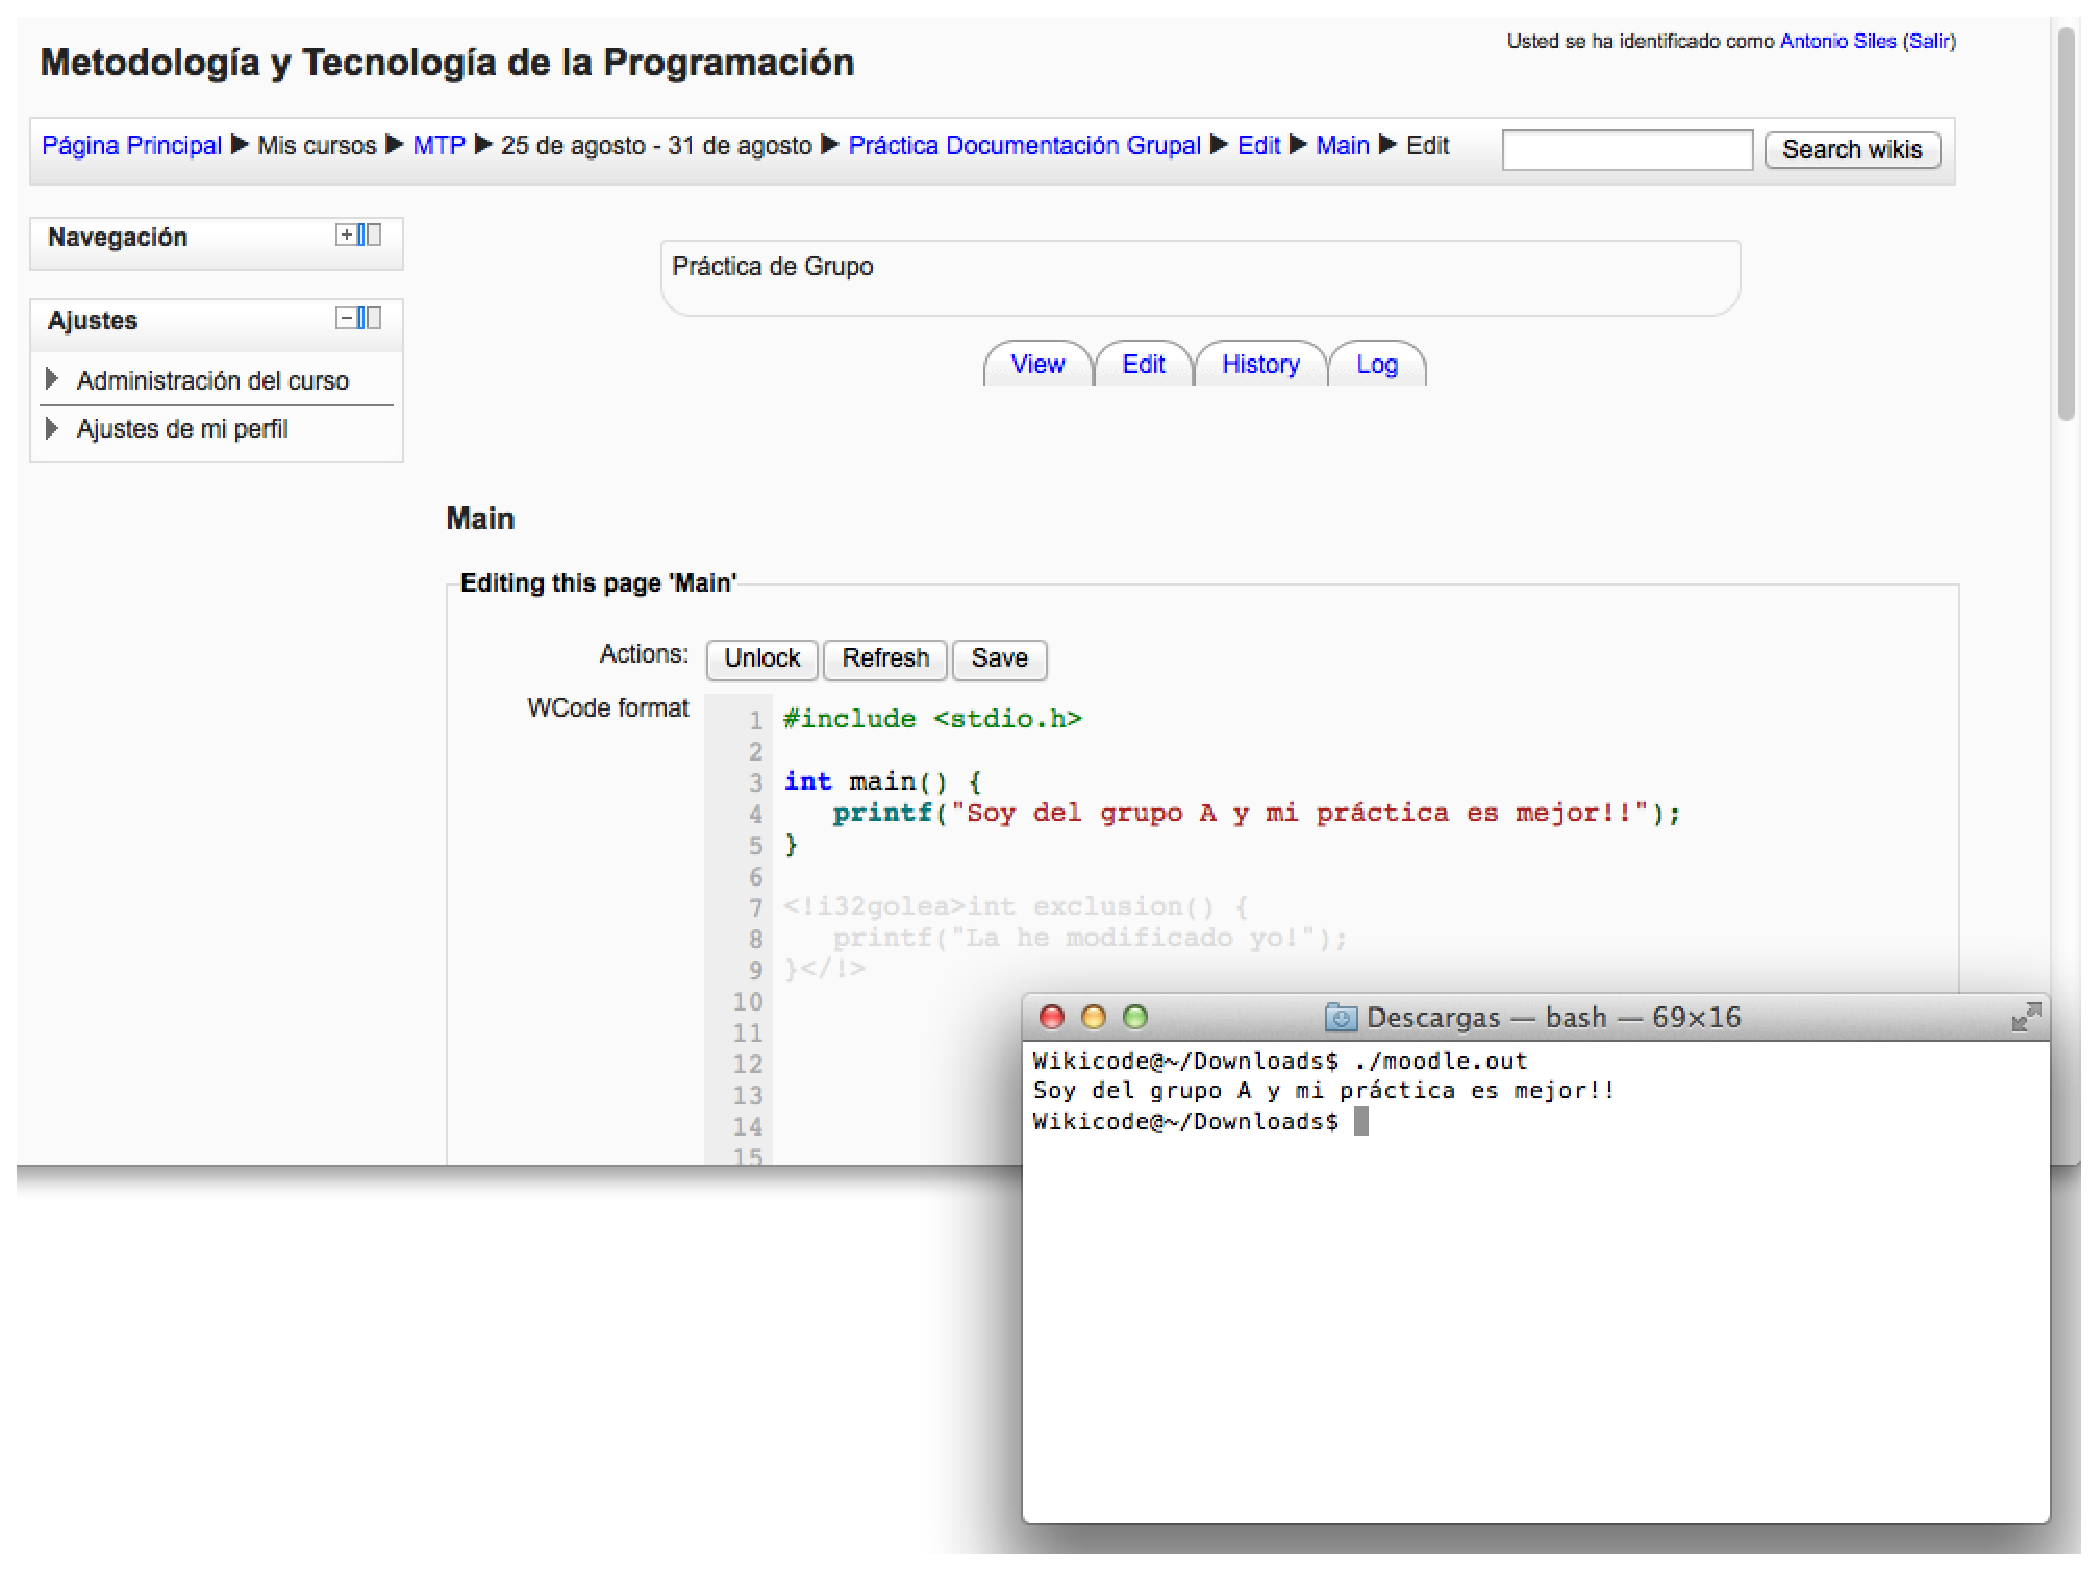
\includegraphics[width=0.9\textwidth]{./img/download.eps}
	\caption{Edición de código. Descarga y ejecución de una aplicación creada.}
\end{figure}	

Por último también se ha comprobado la entrada/salida de texto con respecto al chat que hemos incluido en nuestra plataforma de desarrollo antes de dar el visto bueno a la parte de edición de la plataforma.

\begin{figure}[h]
	\centering
	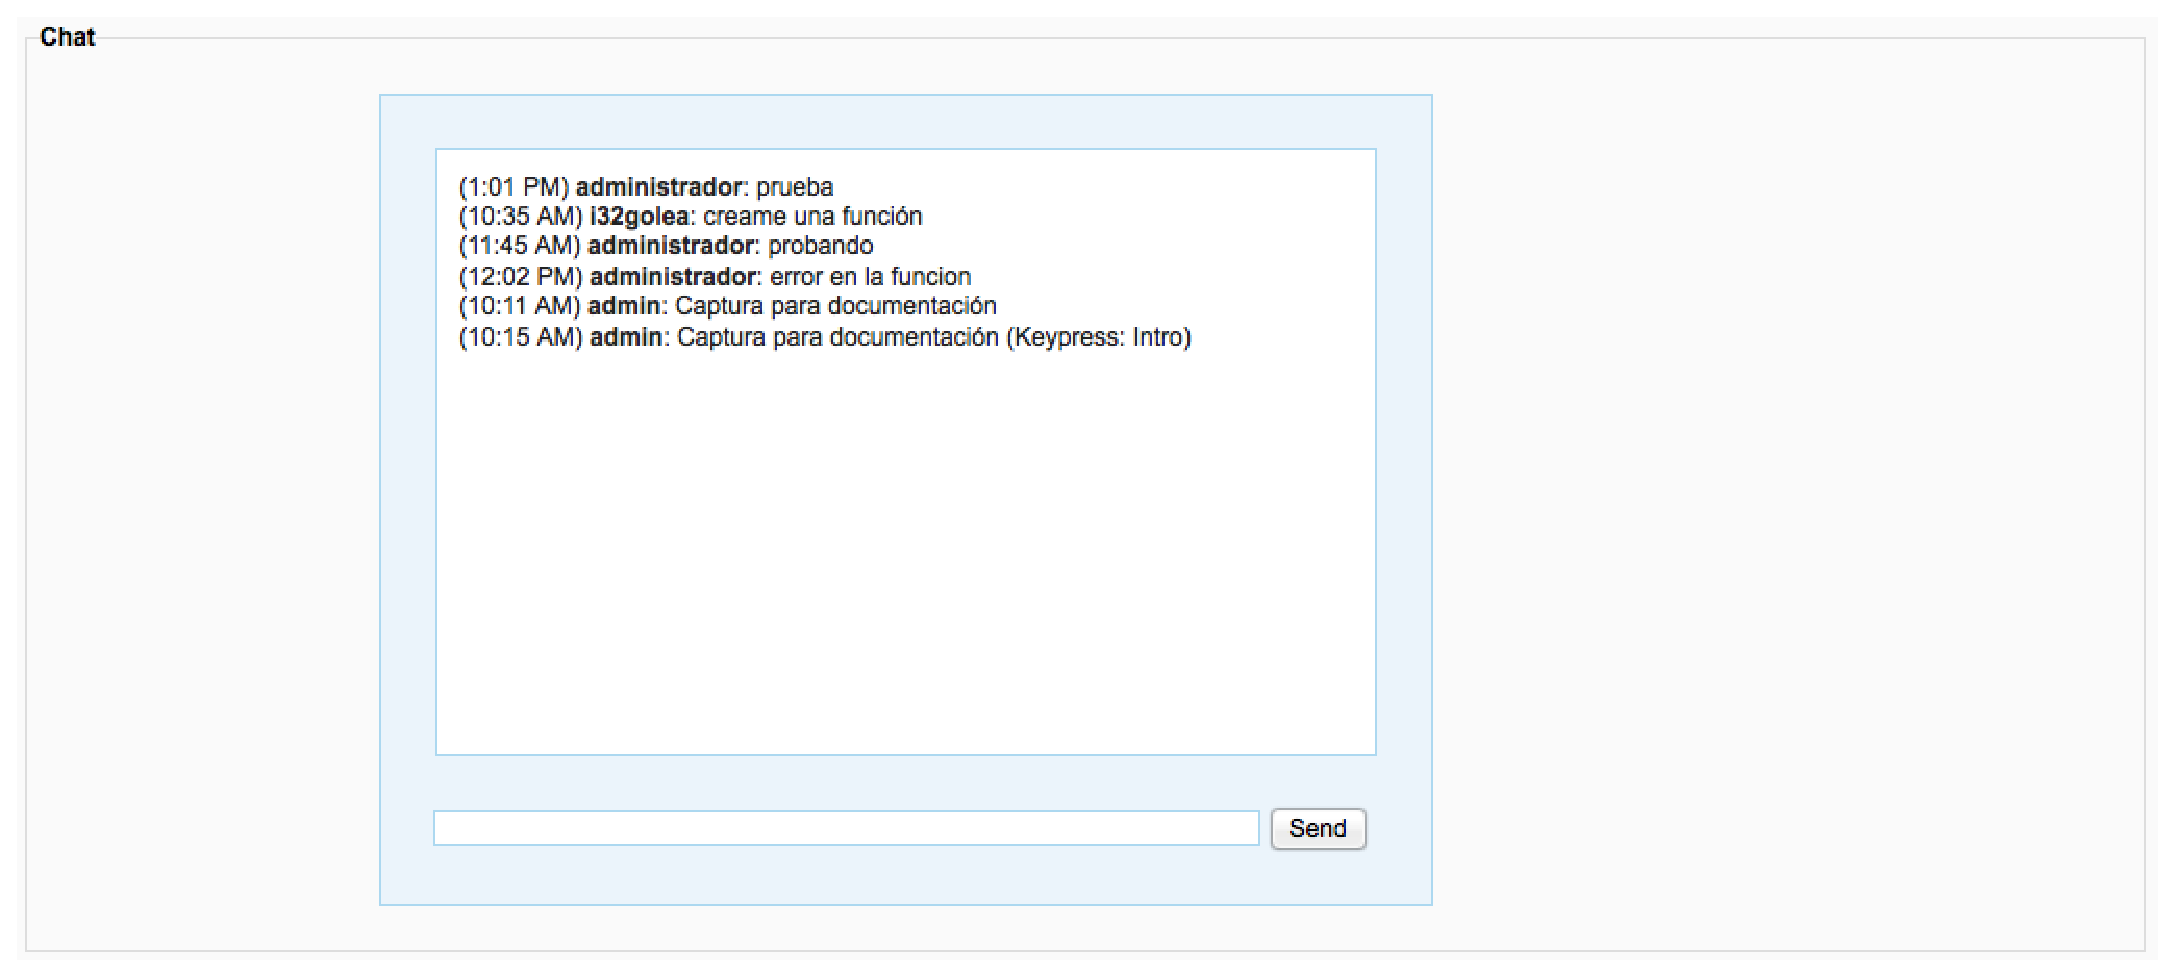
\includegraphics[width=0.65\textwidth]{./img/echat.eps}
	\caption{Edición de código. Chat.}
\end{figure}

\newpage

\subsection{Prueba de compilación utilizando Cross Compiling}
	
Para hacer esta prueba se ha inicializado una máquina virtual con Windows instalado y posteriormente se ha compilado y ejecutado el ejecutable descargado. La salida es la misma que nos ha dado en el sistema operativo nativo de nuestra aplicación por lo que podemos ver que las pruebas realizadas son correctas.
	
\begin{figure}[h]
	\centering
	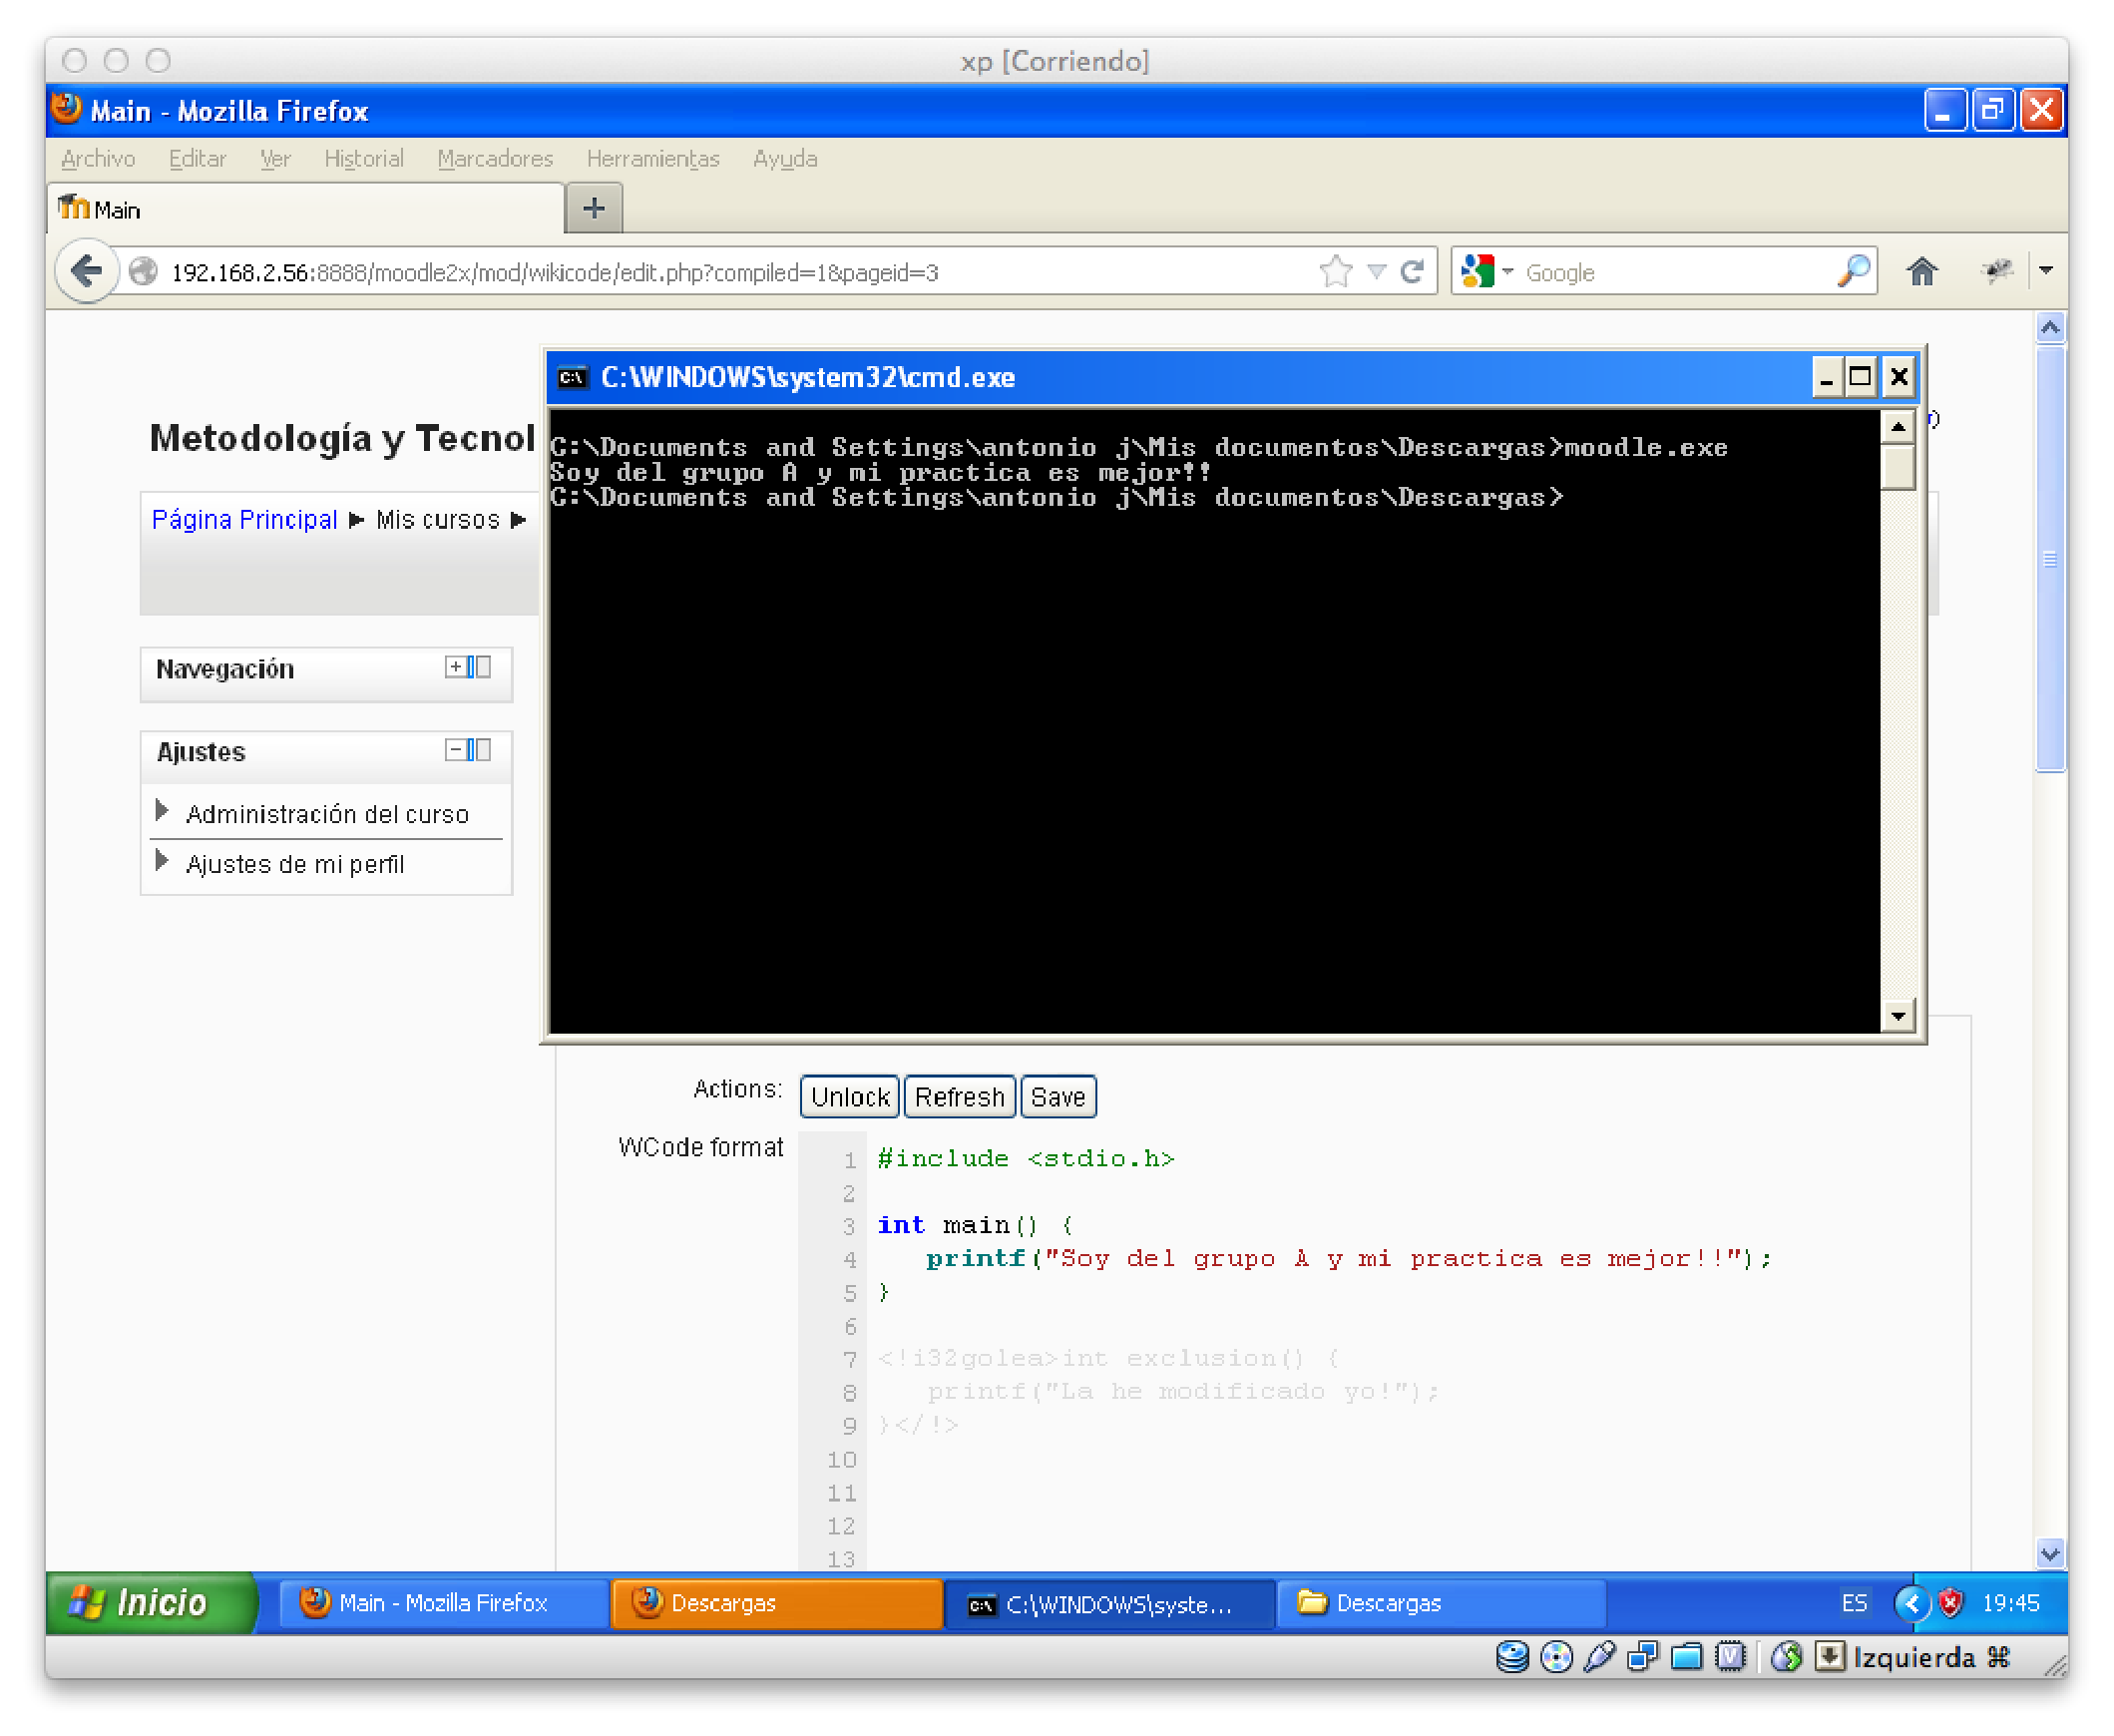
\includegraphics[width=0.9\textwidth]{./img/windows.eps}
	\caption{Edición de código. Cross Compiling.}
\end{figure}		
	
\subsection{Comprobación de estadísticas}
	
Una parte fundamental de Wikicode es su parte estadística, donde el profesor puede comprobar la dificultad que ha tenido un alumno para realizar un determinado código y en función de esto valorar el conocimiento del alumno. Para ello se muestran dos métricas: Número de errores de compilación y Duración de desarrollo del código.

Se han hecho las pruebas oportunas, calculando el tiempo y el número de errores de modo paralelo y comprobando de la veracidad de los hechos.
	
\begin{figure}[h]
	\centering
	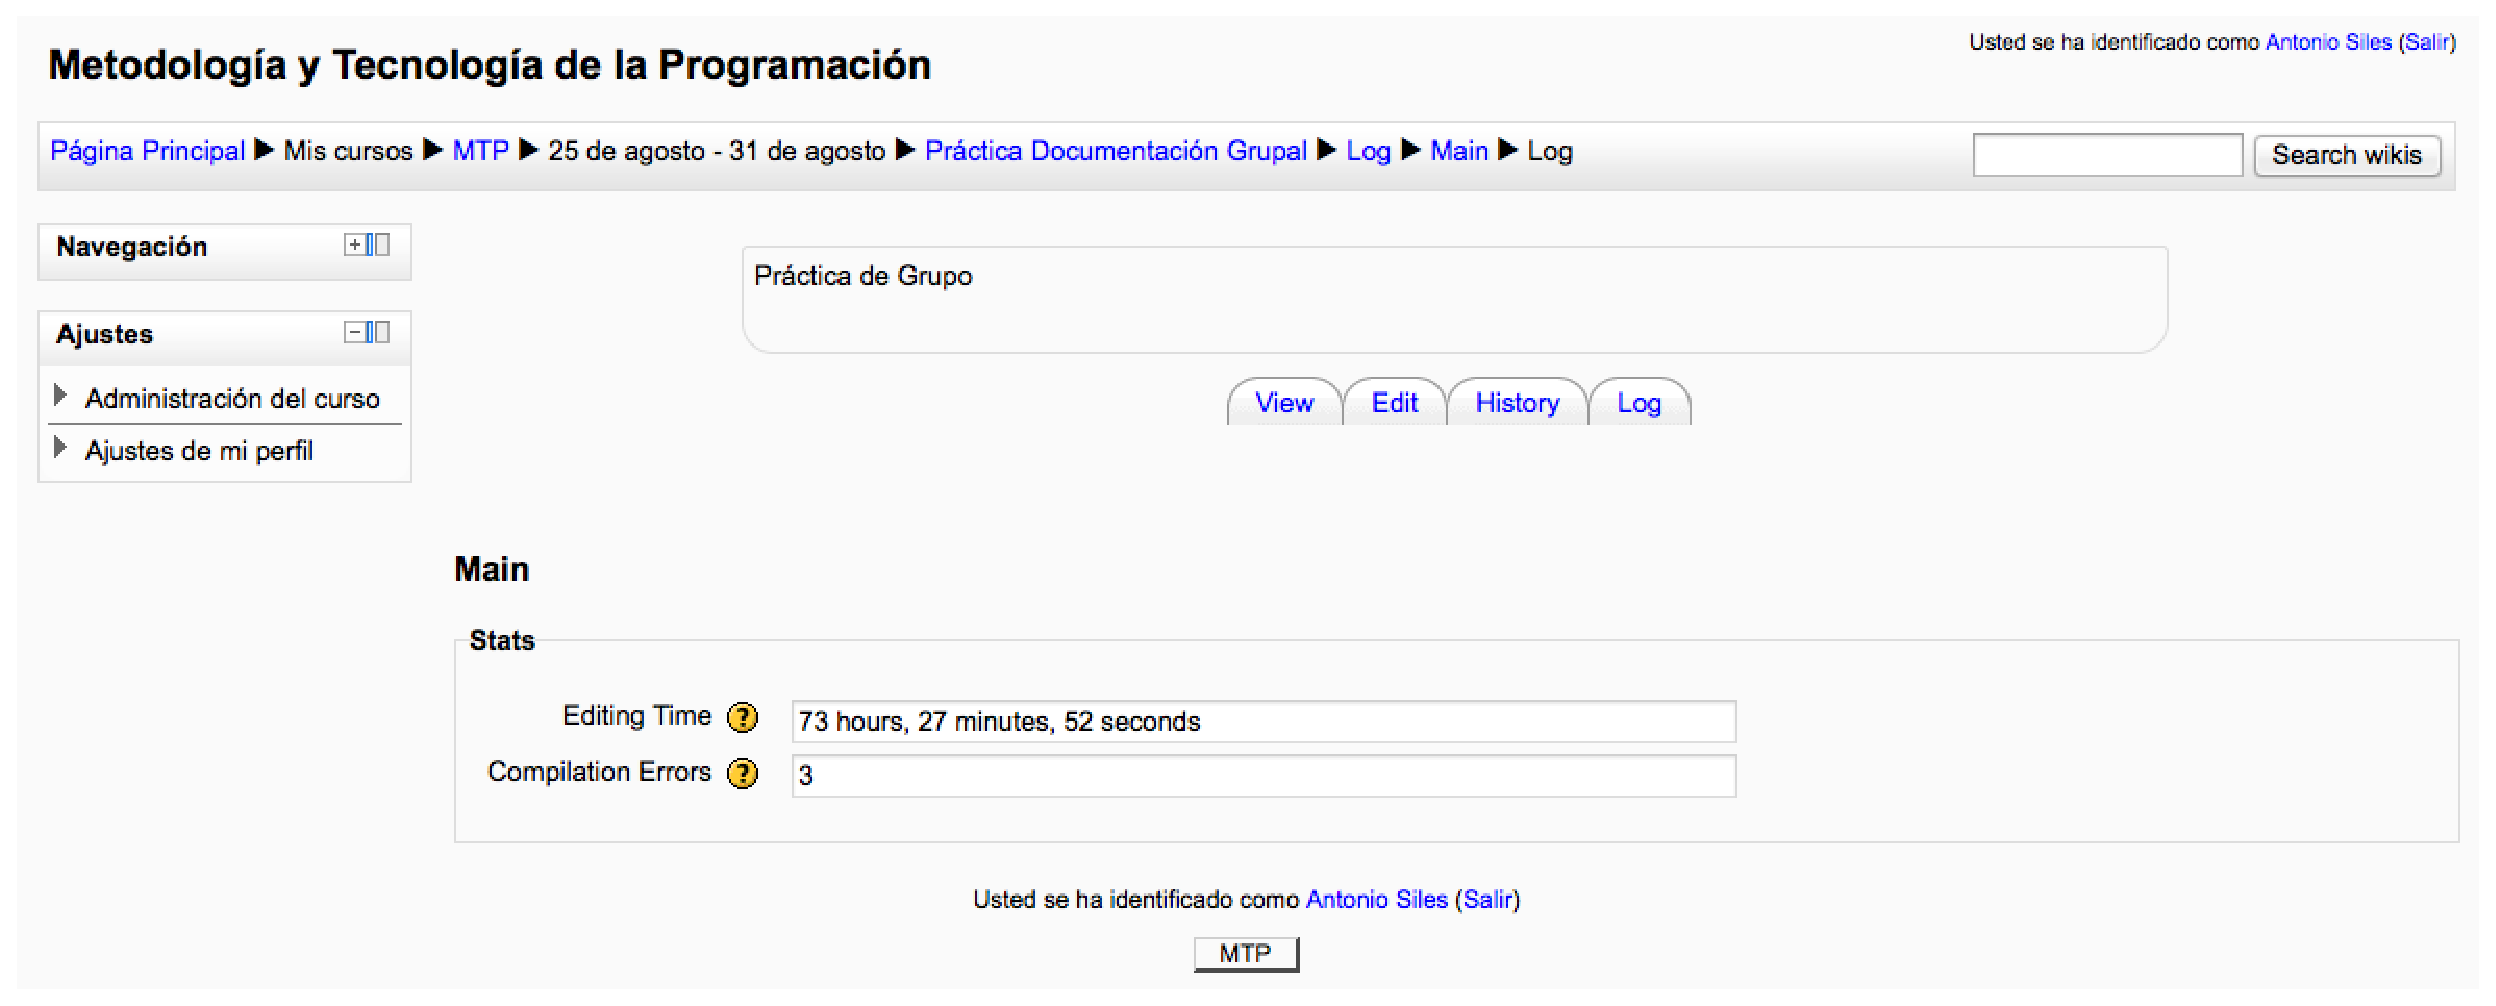
\includegraphics[width=0.9\textwidth]{./img/log.eps}
	\caption{Log de información de una Wikicode.}
\end{figure}

\section{Corrección de errores}

Durante las pruebas se han detectado varios errores de programación, que se han ido corrigiendo conforme se han ido detectando. También se han corregido dos problemas a los que se ha aportado una solución funcional para protección del código, los cuales son los siguientes:

\begin{itemize}
	\item \textbf{Borrado de caracteres especiales}. La aplicación funciona delimitándose por funciones, lo cual nos ayuda a separar los bloqueos unos de otros. Las funciones en el lenguaje de programación C se delimitan por la apertura y cerrado de corchetes, por lo que para eliminar uno de estos caracteres el contenido de su interior ahora deberá de estar vacío. Esto nos impide que el sistema desconozca el dominio de una función.
	\item \textbf{Auto Rollback}. Se ha podido comprobar durante las diversas pruebas que el sistema en caso de error de bloqueos vacía el buffer del código y lo deja en blanco. Se ha modificado la programación de todas las funciones para asegurarnos que siempre que un usuario modifica una función esta esté bloqueada por él, y del mismo modo, por si no se ha detectado algún caso que repercuta en el mismo error se ha programado el sistema de modo que si se vacía el buffer esta acción no se lleve a cabo y restaure el contenido que había anteriormente a la acción que lo ha propiciado.
\end{itemize}

\section{Prueba de aceptación}
	
Esta prueba se ha realizado con varias personas distintas del autor. El uso de la aplicación por parte de esas personas no ha ocasionado ningún error y, por tanto, se puede decir que esta prueba se ha superado de manera satisfactoria.
	
	
	
	
	
	
	
	
	
	
	
	
	
	
	
	
	
	
	
	
	
	
	
	
	
	
	
	
	
	
	
	